\documentclass{article}
\usepackage{graphicx} % Required for inserting images
\usepackage{geometry}
\usepackage{amsmath}
\usepackage{listings}
\usepackage{hyperref}

\title{Analisis y Diseño de Algoritmos}
\author{Marco Antonio Bastida Flores}
\date{13 Junio 2023}

\geometry{left = 30mm, right = 25mm, top = 30mm, bottom = 20mm}

%------------------------------------------------------------------------%

\begin{document}

\maketitle

\section{Quick Sort Algorithm}

\vspace{5mm} %5mm vertical space

%\begin{lstlisting}[language=Python]
\lstinputlisting[language=Python]{Qsort.py}
%\end{lstlisting}

\vspace{5mm} %5mm vertical space

\section{Resultados}

\vspace{5mm} %5mm vertical space

\begin{figure}[ht]
    \centering
    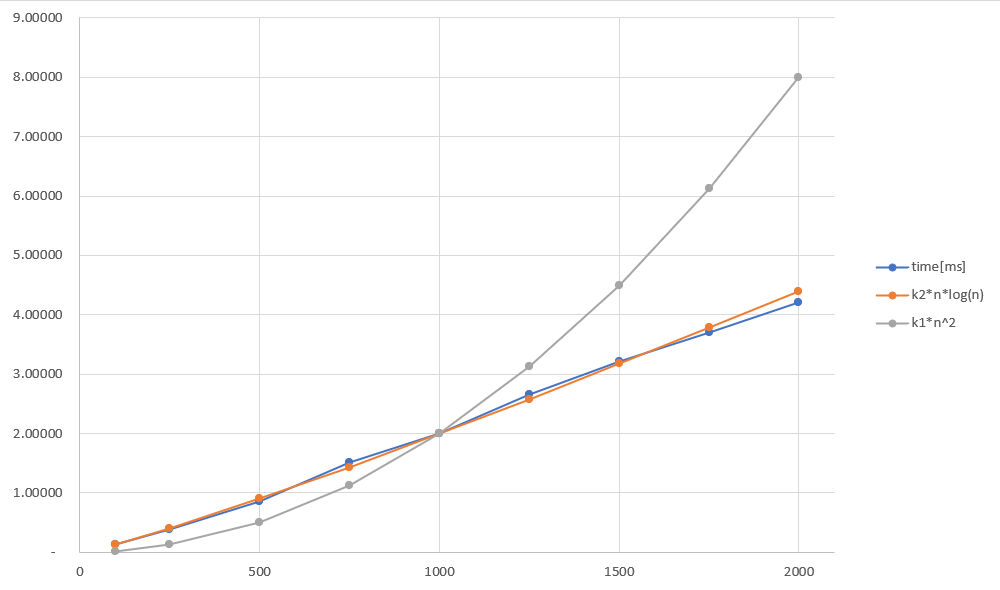
\includegraphics[scale=0.7]{Graph.png}
    \caption{Grafica con resultados y funciones sobrepuestas}
    \label{fig:grafica}
\end{figure}

\vspace{15mm} %5mm vertical space

En la figura \ref{fig:grafica} se muestran que según los resultados de las corridas obtenidas, se aproxima más a un algoritmo \begin{math} n*log(n) \end{math}.

Está manera de analizar algoritmos me pareció bastante interesante, ya que se puede realizar de una manera practica y resulta de una mejor manera mostrar los resultados con una gráfica y así ver más fácil en forma de graficas la comparación de las corridas.

\vspace{15mm} %5mm vertical space

\href{https://github.com/enganthony18/Algorithms}{\includegraphics[scale=0.9]{Git_link.png}}

\end{document}
